%%%%%%%%%%%%%%%%%%%%%%%%%%%%%%%%%%%%%
\subsection{Temperature dependence of the neutron lifespan}\label{sec:neutron}
\para{Understanding neutrons}
Element production during BBN is influenced by several parameters, e.g. baryon to photon ratio $\eta_\gamma$, number of neutrino species $N_\nu$, and neutron to proton ratio $X_n/X_p$, as controlled by both the dynamics of neutron\index{neutron} freeze-out at temperature $T_f\approx 0.8\,\mathrm{MeV}$ and neutron lifetime.

Since about 200 seconds, about 25\% of neutron lifespan, pass between neutron freeze-out, and BBN\index{Big-Bang!BBN} neutron burn at $T\approx0.07\,\mathrm{MeV}$, the in plasma neutron lifetime is one of the important parameters controlling BBN element yields~\cite{Pitrou:2018cgg}. However, the neutron population dynamics and decay within the cosmic plasma medium with large abundances of neutrinos and $e^+e^-$-pairs is not the same as in effective vacuum laboratory environment. The medium influence on particle decay was discussed for example by Kuznetsova et al~\cite{Kuznetsova:2010pi}, we will further develop and use this method in order to explore how cosmic primordial plasma influences neutron population dynamics.
 
After freeze-out when weak interaction scattering processes slow down to allow neutron abundance to free-stream, neutron abundance remains subject to natural decay
\begin{align}\label{Ndec}
n\longrightarrow p+e+\overline{\nu}_e\;.
\end{align}
The current experimental neutron lifetime remains method dependent, with a few seconds discrepancy, we adopt here the value $\tau_n^0=880.2\pm1.0\,\mathrm{sec}$. However measurements using magneto-gravitational traps unlike beam experiments find a bit shorter value, $877.7\pm0.7\,\mathrm{sec}$~\cite{Pattie:2017vsj}. In the standard BBN the neutron abundance when nucleosynthesis begins is assumed to be~\cite{Pitrou:2018cgg}
\begin{align}
\label{Xn_abundance}
X_n(T_{BBN})=X_n^f\exp\left(-\frac{t_{BBN}-t_f}{\tau_n^0}\right)\approx0.13\;.
\end{align}
The normalizing neutron freeze-out yield $X_n^f$ is in terms of abundances 
\begin{align}
\label{Xn_abundance2}
X_n^f \equiv \frac{n_n^f}{n_n^f+n_p^f}= \frac{n_n^f/n_p^f}{1+n_n^f/n_p^f}\;,
\end{align}
where $n_n^f$ and $n_p^f$ are the neutron and proton densities, respectively. The thermal equilibrium yield ratio is, assuming an instantaneous freeze-out
\begin{align}
\label{Xn_abundance3}
 \frac{n_n^f}{n_p^f}= \exp\left(-Q/T_f\right)\;,\qquad Q=m_n-m_p\;.
\end{align}
This value depends on the temperature $T_f$ at which neutrons decouple from the heat bath, and the neutron-proton mass difference (in medium). The values considered in literature are in the range $X_n^f=0.15\sim0.17$~\cite{Pitrou:2018cgg}. A dynamical approach to neutron freeze-out is necessary to fully understand $X_n^f$, we hope to return to this challenge in the near future.

Following freeze-out the neutron is subject to natural decay and normally the neutron lifetime in vacuum $\tau_n^0$ is used to calculate the neutron abundance resulting in the \lq desired\rq\ value $X_n(T_{BBN})\approx0.13$, \req{Xn_abundance} when BBN starts. To improve precision, a dynamically evolving neutron yield needs to be studied and for this purpose we explore here the neutron decay which occurs in medium, not vacuum. This leads to neutron lifespan dependence on temperature of the cosmic medium as the decay occurs for a particle emerged in electron-positron pair plasma and a background of free-streaming neutrinos.

Two physical effects of the medium influence the neutron lifetime in the primordial Universe noticeably:
\begin{itemize}
\item Fermi suppression factors from the medium: 
During the temperature range $T_f\geqslant T\geqslant T_{BBN}$, electrons and neutrinos in the background plasma can reduce the neutron decay rate by Fermi suppression to the neutron decay rate. Furthermore, the neutrino background can still provide the suppression after electron/positron pair annihilation becomes nearly complete.
\item Photon reheating:
When $T\ll m_e$ the electron/positron annihilation occurs, the entropy from $e^\pm$ is fed into photons, leading to photon reheating. The already decoupled (frozen-out) neutrinos remain undisturbed. Therefore, after annihilation we have two different temperatures in cosmic plasma: neutrino temperature $T_\nu$ and the photon and proton temperature $T$ respectively.
\end{itemize}
These two effects will be included in the following exploration of the neutron lifetime in the primordial Universe as a function of $T$. We show how these effects alter the neutron lifespan and obtain the modification of the neutron yield at the time of BBN. Yet another effect was considered by Kuznetsova et al~\cite{Kuznetsova:2010pi} which is due to time dilation originating in particle thermal motion. In our case for neutrons with $T/m<10^{-3}$ this effect is negligible. Below we will explicitly assume that the neutron decay is studied in the neutron rest frame.

%%%%%%%%%%%%%%%%%%%%%%%%%%%%%%%%%%
\para{Decay rate in medium}
%\label{Rate_Medium}
The invariant matrix element for the neutron decay \req{Ndec} for nonrelativistic neutron and proton is given by
\begin{align}
\langle|\mathcal{M}|^2\rangle\approx16\,G^2_FV^2_{ud}\,m_nm_p(1+3g^2_A)(1+RC)E_{\bar{\nu}}E_e,
\end{align}
where the Fermi constant is $G_F=1.1663787\times10^{-5}\,\mathrm{GeV}^{-2}$, $V_{ud}=0.97420$ is an element of the Cabibbo-Kobayashi-Maskawa (CKM)\index{CKM matrix} matrix~\cite{Czarnecki:2018okw,Marciano:2005ec,Czarnecki:2004cw}, and $g_A=1.2755$ is the axial current constant for the nucleons~\cite{Czarnecki:2018okw,Marciano:2014ria}. We also consider the total effect of all radiative corrections relative to muon decay that have not been absorbed into Fermi constant $G_F$. The most precise calculation of this correction~\cite{Marciano:2014ria,Marciano:2005ec} gives $(1+RC)=1.03886$. 

In the primordial Universe the neutron decay rate\index{neutron!lifespan} in medium, at finite temperature can be written as~\cite{Kuznetsova:2010pi}\index{neutron!decay rate in medium}
\begin{align}
\frac{1}{\tau^\prime_n}=\frac{1}{2m_n}\int&\frac{d^3p_{\bar{\nu}}}{(2\pi)^32E_{\bar{\nu}}}\frac{d^3p_p}{(2\pi)^32E_p}\frac{d^3p_e}{(2\pi)^32E_e}(2\pi)^4\delta^4\left(p_n-p_p-p_e-p_{\bar{\nu}}\right)\langle|\mathcal{M}|^2\rangle\notag\\
&\big[1-f_p(p_p)\big]\big[1-f_e(p_e)\big]\big[1-f_{\bar{\nu}}(p_{\bar{\nu}})\big]\;,
\end{align}
where we consider this expression in the rest frame of neutron, \ie\ $p_n=(m_n,0)$. The phase-space factors $(1-f_i)$ are Fermi suppression factors in the medium. The Fermi-Dirac\index{Fermi!distribution} distributions for electron and nonrelativistic proton are given by
\begin{align}
&f_e=\frac{1}{e^{E_e/T}+1},\\
&f_p=e^{-E_p/T}=e^{-m_p/T}\,e^{-p_p^2/2m_pT}.
\end{align}
For neutrinos, after neutrino/antineutrino kinetic freeze-out they become free streaming particles. If we assume that kinetic freeze out occurs at some time $t_k$ and temperature $T_k$, then for $t>t_k$ the free streaming distribution function \req{eq:NeutrinoDist} for antineutrinos is
\begin{align}
f_{\bar{\nu}}=\frac{1}{\exp{\left(\sqrt{\frac{E^2-m_\nu^2}{T_\nu^2}+\frac{m^2_\nu}{T^2_k}}+\frac{\mu_{\bar{\nu}}}{T_k}\right)+1}}\,,\qquad
T_\nu\equiv\frac{a(t_k)}{a(t)}T_k\,,
\end{align}
with the effective neutrino temperature $T_\nu$. In the following calculation, we assume the condition $T_k\gg\mu_{\bar{\nu}},\,m_\nu$, {\it i.e.\/} we consider the massless neutrino in plasma. Substituting the distributions into the decay rate formula and using the neutron rest frame, the decay rate can be written as 
\begin{align}
\label{Decay:Rate_01}
\frac{1}{\tau_n^\prime}&=\frac{G^2_FQ^5V^2_{ud}}{2\pi^3}\,(1+3g^2_A)\,(1+RC)
%\\&\times
\int^1_{m_e/Q}d\xi\,\frac{\xi(1-\xi)^2}{\exp\left(-Q\xi/{T}\right)+1}\frac{\sqrt{\xi^2-(m_e/Q)^2}}{\exp\left(-Q(1-\xi)/T_\nu\right)+1}\,,
\end{align} 
where $Q$ was defined in Eq.\;(\ref{Xn_abundance3}) and we integrate using dimensionless variable $\xi=E_e/Q$. From \req{Decay:Rate_01}, the decay rate in vacuum can be written as
\begin{align}
&\frac{1}{\tau_n^0}=\frac{G^2_Fm_e^5V^2_{ud}}{2\pi^3}(1+3g^2_A)\,(1+RC)\,f^\prime,
\end{align}
where the phase space factor $f^\prime$ is given by
\begin{align}
f^\prime&\equiv\left(\frac{Q}{m_e}\right)^5\int^1_{m_e/Q}d\xi\,{\xi(1-\xi)^2}\sqrt{\xi^2-(m_e/Q)^2}=1.6360\,.
\end{align}

The phase space factor is also modified by the Coulomb correction between electron and proton, proton recoil, nucleon size correction etc. This has been studied by Wilkinson~\cite{Wilkinson:1982hu}, and the phase space factor is given by~\cite{Czarnecki:2018okw,Czarnecki:2004cw,Wilkinson:1982hu}
\begin{align}
f=1.6887.
\end{align}
These effects amount to adding the factor $\mathcal{F}$ to our calculation
\begin{align}
\mathcal{F}=\frac{f}{f^\prime}=1.0322,
\end{align}
then the neutron lifespan can be written as \index{neutron!lifespan in vacuum}
\begin{align}
\tau^{\mathrm{Vacuum}}_n=\frac{\tau^0_n}{\mathcal{F}}=879.481\,\mathrm{sec},
\end{align}
which compares well to the experimental result, $877.7\pm0.7\,\mathrm{sec}$~\cite{Pattie:2017vsj}. 

In the case of plasma medium, we do not expect that these effects (Coulomb correction between electron and proton, proton recoil, nucleon size correction etc) are modified in the cosmic plasma. Thus we adapt the factor into our calculation and the neutron decay rate in the cosmic plasma is given by
\begin{align}
\label{Decay:Rate_02}
\frac{1}{\tau_n^{\mathrm{Medium}}}=&\frac{G^2_FQ^5V^2_{ud}}{2\pi^3}\,(1+3g^2_A)\,(1+RC)\,\mathcal{F}
%\\&\times
\int^1_{m_e/Q}d\xi\,\frac{\xi(1-\xi)^2}{\exp\left(-Q\xi/{T}\right)+1}\frac{\sqrt{\xi^2-(m_e/Q)^2}}{\exp\left(-Q(1-\xi)/T_\nu\right)+1}.
\end{align}
From \req{Decay:Rate_02} we see that the neutron decay rate in the primordial Universe depends on both the photon temperature $T$ and the neutrino effective temperature $T_\nu$.

%%%%%%%%%%%%%%%%%%%%%%%%%%%%%%%%%%%%%%%%%%
\para{Photon reheating}
After neutrino freeze-out and when $m_e\gg T$, the $e^{\pm}$ becomes nonrelativistic and annihilate. In this case, their entropy is transferred to the other relativistic particles still present in the cosmic plasma, {\it i.e.\/} photons, resulting in an increase in photon temperature as compared to the free-streaming neutrinos. From entropy conservation\index{entropy!conservation} we have
\begin{align}
\label{Entropy}
\frac{2\pi}{45}g^s_\ast(T_k)T^3_kV_k+S_{\nu}(T_k)=\frac{2\pi}{45}g^s_\ast(T)T^3V+S_{\nu}(T),
\end{align}
where we use the subscripts $k$ to denote quantities for neutrino freeze-out\index{neutrino!freeze-out} and $g^s_\ast$ counts the degree of freedom for relativistic species in primordial Universe. After neutrino freeze-out, their entropy is conserved independently and the temperature can be written as
\begin{align}
T_\nu\equiv\frac{a(t_k)}{a(t)}T_k=\left(\frac{V_k}{V}\right)^{1/3}T_k.
\end{align}
In this case, from entropy conservation, \req{Entropy}, we obtain
\begin{align}
\label{Neutrino_Photon}
T_\nu=\frac{T}{\kappa},\,\,\,\,\,\,\kappa\equiv\left[\frac{g^s_\ast(T_k)}{g^s_\ast(T)}\right]^{1/3}.
\end{align}
From \req{Neutrino_Photon} the neutron decay rate in a heat bath can be written as
\begin{align}
\label{Decay:Rate_03}
\frac{1}{\tau_n^\mathrm{Medium}}=&\frac{G^2_FQ^5V^2_{ud}}{2\pi^3}(1+3g^2_A)\,(1+RC)\,\mathcal{F}
%\\&\times
\int^1_{m_e/Q}d\xi\,\frac{\xi(1-\xi)^2}{\exp\left(-Q\xi/{T}\right)+1}\frac{\sqrt{\xi^2-(m_e/Q)^2}}{\exp\left(-Q(1-\xi)\kappa/T\right)+1}. 
\end{align}

In the high temperature regime, $T\gg Q$, the exponential terms in the Fermi distribution becomes $1$ and the decay rate is given by
\begin{align}
&\frac{1}{\tau_n^\mathrm{Medium}}=\frac{1}{4}\left(\frac{1}{\tau_n^\mathrm{Vacuum}}\right)\;,
\qquad
T\gg Q\;.
\end{align}
In \rf{Decay:Rate} on the left-hand side we show the  neutron lifetime $\tau^\mathrm{Medium}_n$ in plasma as a function of temperature. Fermi-suppression from electron and neutrino increases the neutron lifetime as compared to value in vacuum. At low temperature, $T<0.2\,m_e$, most of the electrons and positrons have annihilated and the main Fermi-blocking comes from the cosmic neutrino background. In this regime, the neutron lifetime depends also on the neutrino temperature, $T_\nu$. For cold neutrinos $T_\nu<T$, the Fermi suppression is smaller than the hot one $T_\nu=T$, the effect is made more visible in the insert.

%%%%%%%%%%%%%%%%%%%%%%%%%%%%%%%%%%%%%%%%%%%%%%%%%%%%%%%%%%%%%%%%%
\begin{figure} 
\centerline{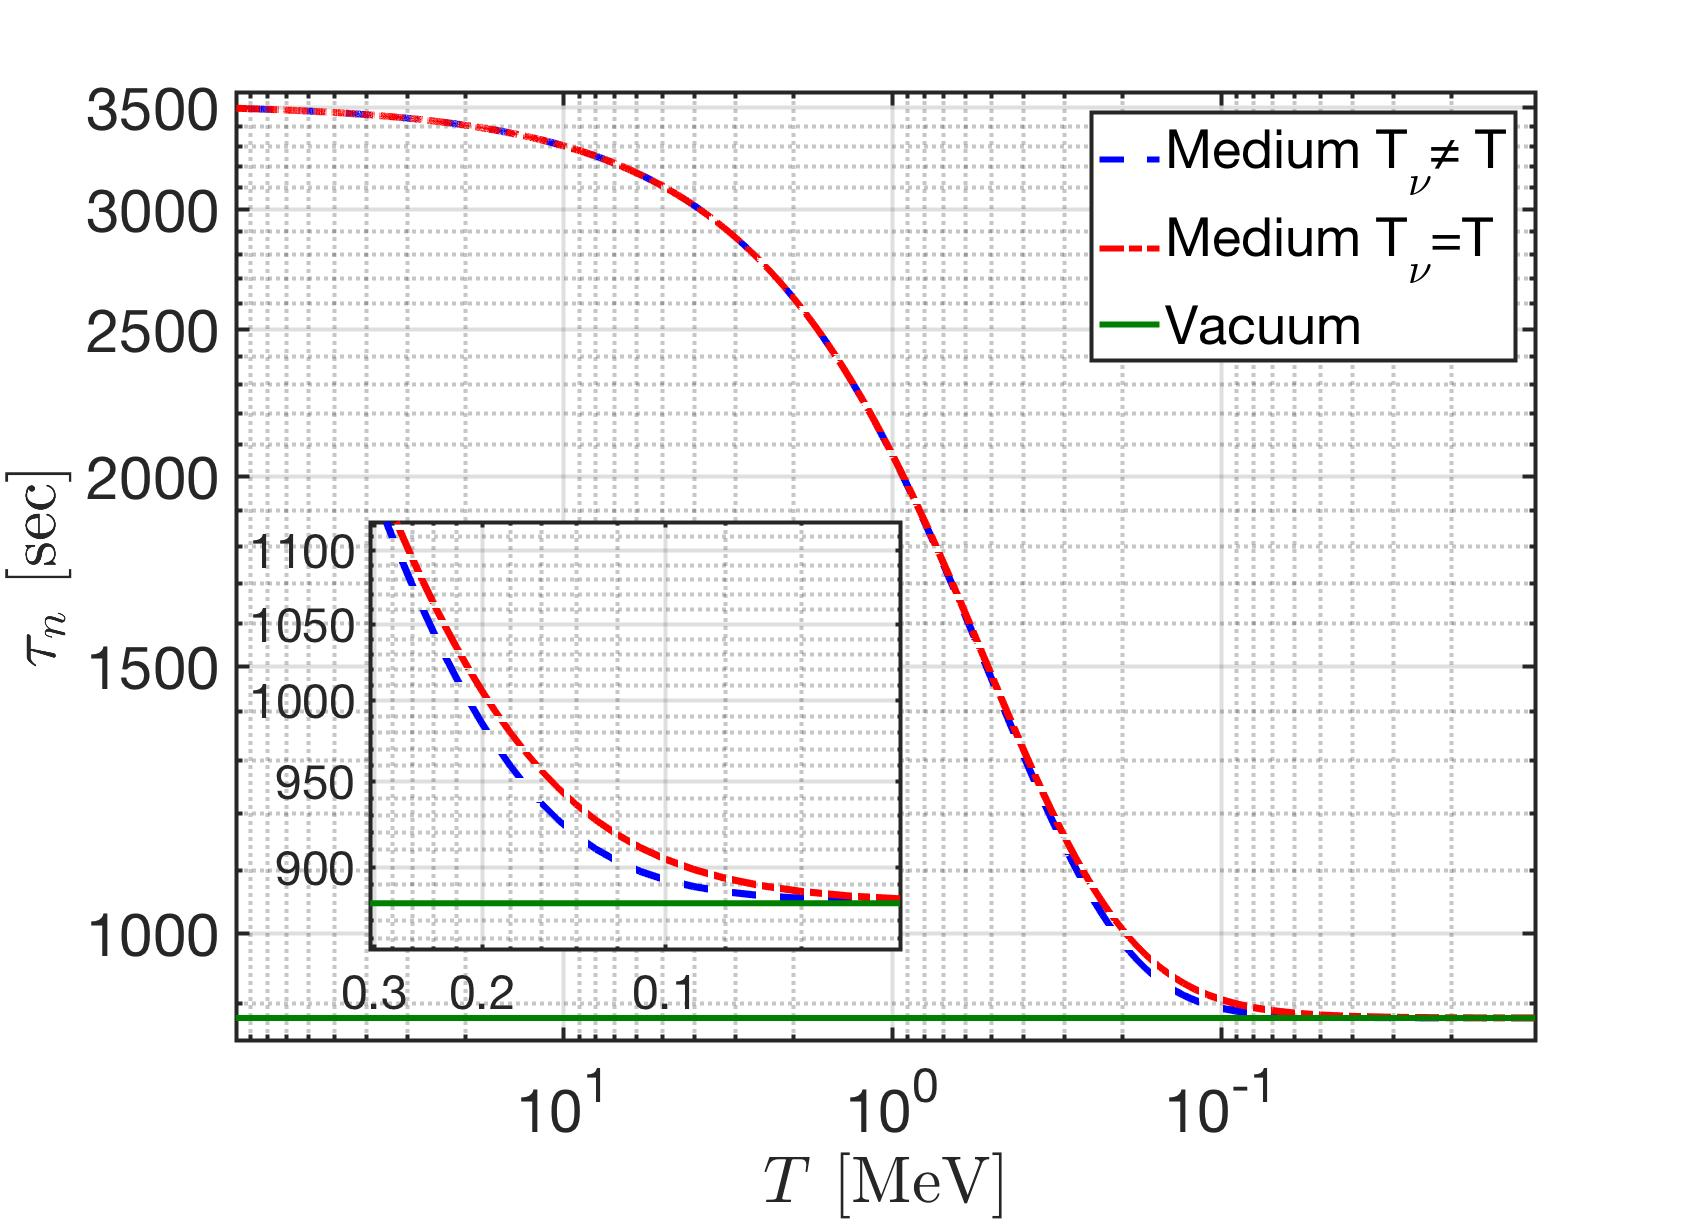
\includegraphics[width=0.5\linewidth]{./plots/Neutron_Lifetime_001}\hspace*{-0.5cm}
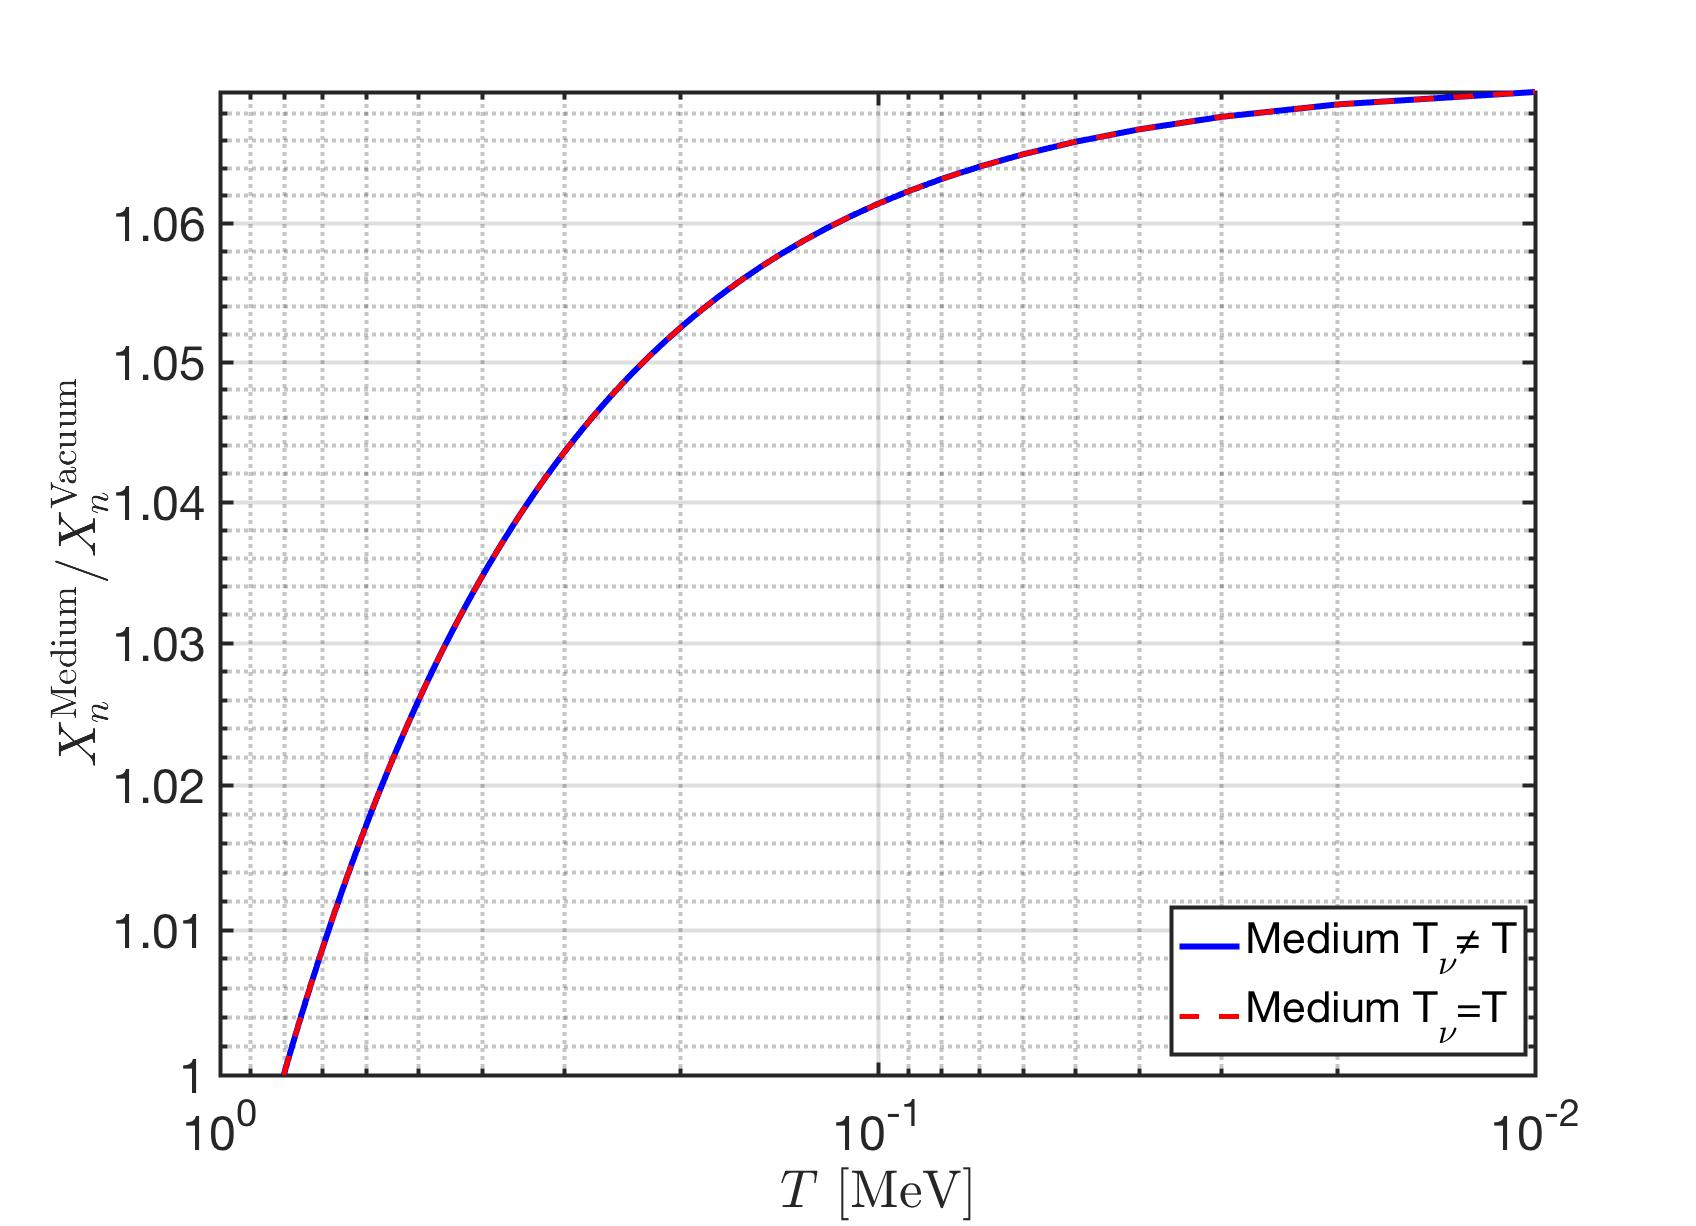
\includegraphics[width=0.5\linewidth]{./plots/Neutron_Abundance}}
\caption{On left: The neutron lifetime $\tau_n^\mathrm{Medium}$ in the cosmic plasma; On right: The neutron abundance in the cosmic plasma, ratio to vacuum  abundance, as a function of temperature\cccite{Yang:2018qrr}}
\label{Decay:Rate}
\end{figure}
%%%%%%%%%%%%%%%%%%%%%%%%%%%%%%%%%%%%%%%%%%%%%%%%%%%%%%%%%%%%%%%%%% 

%%%%%%%%%%%%%%%%%%%%%%%%%%
\para{Neutron abundance}
After the neutron freeze-out, the neutron abundance is only affected by the neutron decay. The neutron concentration can be written as \index{neutron!particle abundance}
\begin{align}
\label{Abundance}
X_n=X_n^f\,\exp\bigg[-\int^t_{t_f}\frac{dt^\prime}{\tau_n}\bigg],
\end{align}
where we use the subscripts $f$ to denote quantities at neutron freeze-out. Using \req{Decay:Rate_03} and \req{Abundance}, the neutron abundance ratio between plasma medium and vacuum is given by
\begin{align}
\label{Abundance_Ratio}
\frac{X_n^{\mathrm{Meduim}}}{X_n^{\mathrm{Vacuum}}}=\exp\bigg[-\int^t_{t_f}dt^\prime\left(\frac{1}{\tau^\prime_n}-\frac{1}{\tau^0_n}\right)\bigg].
\end{align}

On the right-hand side in \rf{Decay:Rate}  we show this neutron abundance ratio as a function of temperature. We consider as typical the neutron freeze-out temperature $T_f=0.08\mathrm{MeV}$ and the BBN  temperature $T_{BBN}\approx0.07\mathrm{MeV}$, which yields ${X_n^{\mathrm{Meduim}}}/{X_n^{\mathrm{Vacuum}}}=1.064$. Then from \req{Xn_abundance} the neutron abundance in plasma medium is given by
\begin{align}
X_n^{\mathrm{Meduim}}=1.064\,X_n^{\mathrm{Vacuum}}\approx0.138.
\end{align}
In this case, the neutron abundance will increase about $6.4\%$ in the cosmic plasma which should affect the final abundances of the Helium-4 and other light elements in BBN. A further study of neutron decoupling and decay in medium will be needed. 
 
%%%%%%%%%%%%%%%%%%%%%%%%%%%%%%%%%%%%%%%%%%%%%%%%%%
%%%%%%%%%%%%%%%%%%%%%%%%%%%%%%%%%%%%%%%%%%%%%%%%%%%%%%%%%%%%%%%%%%
\para{How is BBN impacted?}
One of the important parameters of standard BBN is the neutron lifetime, as it affects the neutron abundance after neutron freeze-out at temperature $T_f\approx 0.8 \mathrm{MeV}$ and before the BBN $T\approx0.07 \mathrm{MeV}$. 

In the standard BBN model, it is necessary to have a neutron-to-proton ratio $n/p\approx1/7$ when BBN begins in order to explain the observed values of hydrogen and helium abundance~\cite{Pitrou:2018cgg}. We have evaluated the effect of Fermi suppression on the neutron lifetime due to the background electron-positron  and free-streaming neutrino plasma. We found that in a very hot medium ($T>10$\,MeV) the neutron lifetime is lengthened by up to a factor 4. Our method should in principle also be considered in the study of medium modification of just about any of the relevant weak interaction rates which in this report we used as given in vacuum,  this remains a task for another day.

In the temperature range between neutron freeze-out just below $T=1$\;MeV and BBN conditions the effect of neutron lifespan is smaller but still quite noticeable. Near neutron freeze-out both decay electron and neutrino are blocked. However, after $e^\pm$ annihilation is nearly complete  Fermi-blocking comes predominantly from the cosmic neutrino background and the neutron lifetime depends on the temperature $T_\nu<T$.

We found that the increased neutron lifetime results in an increased neutron abundance ${X_n^{\mathrm{Meduim}}}/{X_n^{\mathrm{vacuum}}}=1.064$ at $T_{BBN}\approx0.07 \mathrm{MeV}$ \ie\ we find a $6.4\%$ \emph{increase} in neutron abundance due to the medium effect at the time of BBN. We believe that this effect needs to be accounted for in the precision BBN study of the final abundances of heavy hydrogen, helium and other light elements produced in BBN.
